\def \Subject {تمرین  اول}
\def \Course {درس امنیت}
\def \Author {ملیکا محمدی فخار - ستاره باباجانی}
\def \Report {گزارش تمرین}
\def \StudentNumber {99522086 - 99521109}



\begin{center}
\vspace{.4cm}
{\bf {\huge \Subject}}\\
\vspace{.6cm}
{\bf \Large \Course}\\
{\Large \Report} \\
\vspace{.3cm}
{\bf \Author }  \\
\vspace{.2cm}
{\bf \ \StudentNumber}\\\

\end{center}

\hspace{\fill} 

\clearpage



\section{جواب سوال 1}
همانطور که می دانیم، حمله ی force Brute یا جستجوی فراگیر نوعی از حملات است که در آن تمامی  ترکیب های ممکن از حروف یک گذرواژه تا زمان یافتن رمز اصلی امتحان می شوند. البته که حجم بالایی از رخدادهای نفوذ اطلاعاتی در دهه نود شمسی با استفاده از این رویکرد انجام گرفته است، اما فرایند رمزنگاری با استفاده از این حمله ازجمله فرایندهای طولانی به حساب می آید. البته که اینجور کارها عمدتا به کامپیوترها سپرده می شود تا فرایند امتحان کردن حالات مختلف را به صورت خودکار انجام دهند. 

انواع مختلفی از این نوع حملات 

•	حملات ساده (simple Brute Force Attacks) 

•	حملات معکوس (Reverse Brute Force Attacks)

•	حملاتی از نوع دستکاری اعتبار (Credential Stuffing)  

•	حملات دیکشنری (Dictionary Attacks)

•	حملات هیبریدی Attacks)   (Hybrid 

منابع مورد نیاز این حمله با افزایش طول کلید به صورت خطی افزایش پیدا نمی کنند. بلکه بصورت  نمایی افزایش می یابند. بدیهی است انتخاب رمزهای طولانی تر و پیچیده تر، عملیات Brute force را وادار به آزمایش موارد بیشتری می کند که زمان موردنیاز برای بررسی تمام حالت ها نیز افزایش می یابد. 
چند نمونه از ابزارهای رایج که از این حمله استفاده می کنند را می توان به صورت زیر اشاره کرد: 

•	Rainbow crack

•	John the ripper

•	Aircrack-ng

به عنوان نمونه، چند مزیت و دلیل برای استفاده از ابزار John the Ripper را می توان در تصویر زیرمشاهده نمود:

\begin{figure}[ht!]
    \centering
    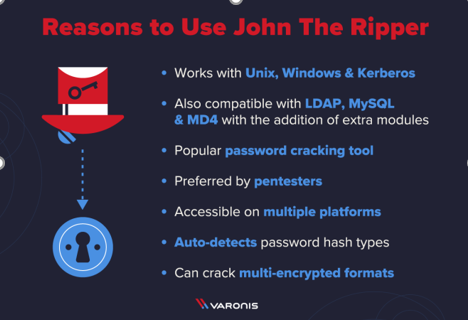
\includegraphics[width=0.5\linewidth]{images/image.png}
    \caption{مزیت و دلیل استفاده از John the Ripper}
    \label{fig:dynamicprogramming}
\end{figure}

با توجه به اطلاعات آماری جمع آوری شده حدود ۵درصد از حملات سایبری از نوع Brute-force هستند که درصد بسیار پایینی است.
معمولا سیستم های حمله کننده می توانند حدود ۱۰هزار تا یک میلیارد رمز را در ثانیه آزمایش کنند
که بستگی که پردازنده و سخت افزار سیستم حمله کننده دارد.

زمان مورد نیاز برای پیدا کردن یک رمز به موارد زیر بستگی دارد:

•	تعداد کاراکترهای به کاررفته در رمز

•	تنوع حروف به کاررفته در رمز

•	 قدرت رمز سیستم حمله کننده

•	 قدرت رمز سیستم هدف


بود. در یک کیبورد استاندارد حدود ۹۴ کاراکتر داریم که در مجموع می توانند ۲میلیارد رمز ۸ حرفی به وجود بیاورند که تعداد حالات بسیار زیادی هست و چک کردن تمام این حالت ها زمانبر هست. به طور کلی می توانیم بگوییم با افزایش طول رمز، سرعت شکستن آن رمز به طور نمایی افزایش پیدا می کند و رشد می کند. به عنوان نمونه، شکستن رمزی با تعداد ۱۲۸بیت با استفاده از این روش، نیاز به بررسی \(2^{128}\) حالت دارد که میلیاردها سال طول خواهد کشید. \\ \\

\(**\) نمونه از مدل‌های پرقدرت CPU :\\
\textbf{i9-11900K Core :Intel}\\
یکی از پرقدرت‌ترین پردازنده‌های مرکزی از شرکت Intel  
دارای 8 هسته و 16 رشته اجرایی است.
 این دستگاه می تواند حدود 1700 به بالا امتیاز (در قسمت  Score Single-Core 5 Geekbench (Benchmark: کسب کند.\\
\textbf{5950X 9 Ryzen :AMD}\\
یک پردازنده قدرتمند از شرکت  AMD
دارای 16 هسته و 32 رشته اجرایی است.
این دستگاه می تواند حدود 25000 به بالا امتیاز (در قسمت Score Single-Core 5 Geekbench (Benchmark کسب کند. \\ \\
\(**\) نمونه از مدل‌های پرقدرت :GPU   \\
\textbf{3090 RTX GeForce :NVIDIA}\\
یک کارت گرافیکی بسیار پرقدرت از NVIDIA
دارای 10,496 هسته CUDA و 24 گیگابایت حافظه GDDR6X است.
این دستگاه می تواند حدود 15000 به بالا امتیاز (در قسمت Benchmark: 3DMark Time Spy ) کسب کند. \\
\textbf{XT 6900 RX Radeon :AMD}\\
یکی دیگر از کارت‌های گرافیکی قدرتمند از AMD 
دارای 5,120 هسته جریانی و 16 گیگابایت حافظه GDDR6 است.
این دستگاه می تواند حدود 11000 به بالا امتیاز (در قسمت Optimized 8k Superposition Unigine Benchmark: ) کسب کند.


\section{جواب سوال 2}

الگوریتم Transposition Double یکی از الگوریتم‌های رمزنگاری کلاسیک بوده است که توسط آلمان در طول جنگ جهانی اول I) War (World مورد استفاده قرار می‌گرفت. این الگوریتم از مبانی ساده‌ای برای رمزنگاری متن استفاده می‌کند و از ترتیب دو مرحله‌ای برای انجام عملیات رمزنگاری و رمزگشایی تشکیل شده است. \\
توضیح مختصر الگوریتم Transposition Double به شرح زیر است:

\subsection{مرحله ی اول : رمزنگاری  Transposition :Row}
1. متن اصلی را به یک جدول با ستون‌ها و ردیف‌ها تبدیل می‌کند. \\
2. ردیف‌های جدول را بر اساس کلید مشخص مرتب می‌کند. \\
3. متن رمزگشایی شده را به صورت ردیف به ردیف خوانده و بازیابی می‌کند. 

\subsection{مرحله ی دوم: رمزنگاری  Transposition :Column}
1. متن اصلی را به یک جدول با ستون‌ها و ردیف‌ها تبدیل می‌کند. \\
2. ستون‌های جدول را بر اساس کلید مشخص مرتب می‌کند. \\
3. متن رمزگشایی شده را به صورت ستون به ستون خوانده و بازیابی می‌کند. 

\subsection{مرحله ی سوم: رمزنگاری و رمزگشایی:}
برای رمزنگاری یک متن، متن اصلی به مرحله اول و سپس به مرحله دوم تبدیل می‌شود.
برای رمزگشایی، مراحل برعکس انجام می‌شوند.
الگوریتم Transposition Double به عنوان یکی از الگوریتم‌های رمزنگاری ساده و قدیمی شناخته می‌شود و مزایای مختصری دارد. از جمله مزایا می‌توان به سادگی اجرا و قابلیت تنوع کلید اشاره کرد. با این حال، امروزه این الگوریتم به عنوان یک الگوریتم امن برای استفاده در موارد مهم و حساس معمولاً مورد تایید نیست. الگوریتم‌های رمزنگاری پیشرفته‌تر و امن‌تری برای حفظ امنیت اطلاعات استفاده می‌شوند.


\section{جواب سوال 3}

این روش برای شکستن رمزنگاری های جانشینی بسیار مناسب است. مبنای کار آن تکرار حروف در الفبای انگلیسی است. ابتدا تکرار هر حرف الفبا در متن رمزه شده را به دست می آوریم. سپس تکرار حروف الفبای انگلیسی در متن های بزرگ را به دست می آوریم و براساس تعداد تکرار مرتب میکنیم. سپس میان این دو لیست یک نگاشت برقرار میکنیم.
این روش تا حد خوبی میتواند مسئله ما را رمزگشایی کند. اما به جواب مطلق درست نخواهد رسید.
در روش رمز نگاری مستوی، هر حرف با یک ضرب و جمع با عدد، به یک حرف دیگر نگاشت خواهد شد. البته بعد از ضرب و سپس جمع، باید باقیمانده عدد حاصل را بر 26 محاسبه کنیم تا حرفی از بین حروف الفبای انگلیسی بدست آید.
برای انجام این کار ابتدا یک دیکشنری که کلید آن جفت (a,b) است و هرvalue آن لیستی از کلمات رمز گشایی شده است ساخته میشود. سپس برای تمام مقادیر ممکن aو b متن را رمزگشایی میکند و با استفاده از کتاب خانه های موجود (که برای زبان پایتون از nltk استفاده میکنیم) کلمات معنادار پیدا میشوند. و کلمات معنادار به دیکشنری اضافه میشوند.
نتیجه بعد از تست همه حالات به صورت زیر است:
\begin{figure}[ht!]
    \centering
    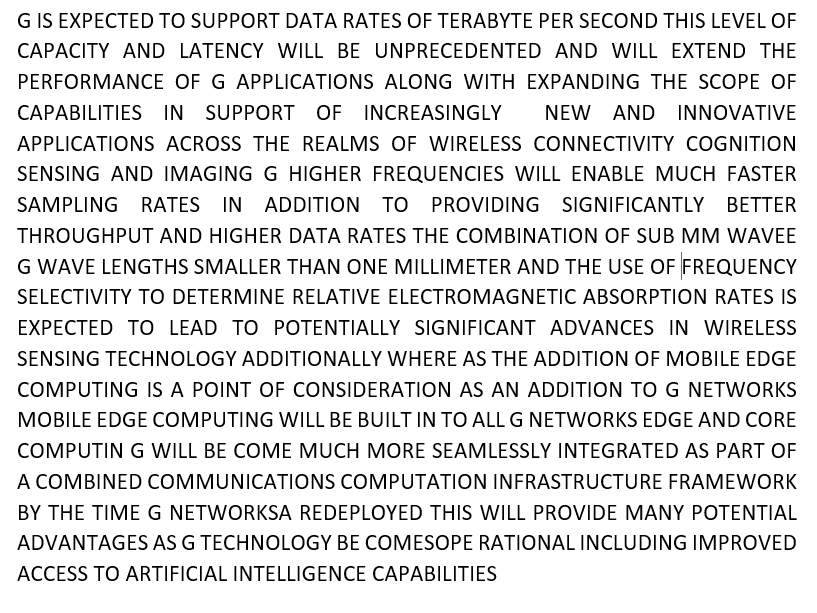
\includegraphics[width=1.1\linewidth]{images/text.png}
  
    \label{fig:dynamicprogramming}
\end{figure}